\section{Distributed Smart Space Orchestration System}
\label{sec:ds2os}

Distributed Smart Space Orchestration System (DS2OS) is a framework that allows orchestration of a collection of smart devices together to create different types of intelligent smart environments \cite{pahl2014distributed}. 

DS2OS consists of three main building blocks:

\begin{enumerate}
  \item The Virtual State Layer (VSL) \si{\micro}-middleware (Middle Layer).
  \item The Service-to-Space (S2S) service management framework.
  \item The Smart Space Store (S2Store).
\end{enumerate}

\textbf{The Virtual State Layer (VSL) \si{\micro}-middleware} is introduced in \cite{pahl2013missing}\cite{pahl2014distributed}. Virtual State Layer (VSL) is a representation that allows abstraction of smart devices and their orchestration to form smart spaces. VSL virtualizes the real world of sensors and actuators in a software environment called ``middleware''. A middleware then facilitates creation of softwares that can easily use these abstract representations to create advanced smart spaces.

Traditionally middlewares are domain specific: they cater to domain specific devices and domain specific orchestration scenarios. Pahl calls the domain specific middlewares as \emph{silos}. These silos lack interoperability and reuse. E.g., an intrusion detection system for a large warehouse and similar system for home automation are likely to use different middleware systems although they share similar requirements.

VSL as a \si{\micro}-middleware differs from other smart space middlewares because it is not limited to any specific domain.

VSL requires that hardware devices are abstracted into meta devices called \emph{context models} based on their utility. Hardware devices with similar features but different vendors can share the same context model. Hardware devices are linked with their respective context models in VSL by device specific software called gateway services.

VSL then provides features that allow any software system to communicate with the context models, thus decoupling a software system from the hardware device.

\textbf{The Service-to-Space (S2S) service management framework} provides a set of functionalities related to service management like service installation, uninstallation, starting, pausing, stopping and monitoring running services. Analogous to a mobile operating system that provides the necessary conditions to run mobile apps, the service management framework can run services developed for DS2OS. S2S handles services running in an environment consisting of distributed computing hosts.

\textbf{The Smart Space Store (S2Store)} is a web-based app Store that contains repositories for context models, access groups and services. It is a market for users to download applications suitable for their smart spaces. Users can provide feedback and/or rate applications. Developers can search and download existing context models and access groups and reuse them. User feedbacks as well as usage statistics of existing entities are used to calculate reputation for these entities.

The reputations are the central part of this thesis as we see the importance of their roles in Section \ref{sec:s2store_ecosystem}.

\begin{landscape}

  \begin{figure}
    \centering
    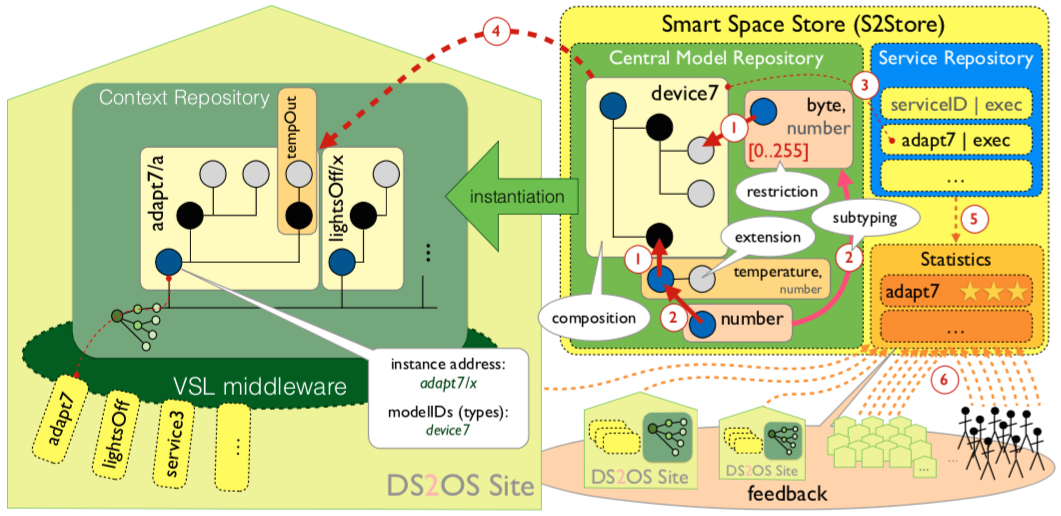
\includegraphics[width=21cm]{figures/ds2os.png} 
    \caption{Overview of DS2OS. (Source~\cite{pahl2014distributed})}
    \label{fig:ds2os}
  \end{figure}

\end{landscape}
